%%%%%%%%%%%%%%%%%%%%%%%%%%%%%%%%%%%%%%%%%%%%%%%%%%%%%%%%%%%%%%%%%%%%%%%%%%
%% Review Volume (last updated on 20-4-2015)                            %%
%% Trim Size: 9in x 6in                                                 %%
%% Text Area: 7.35in (include runningheads) x 4.5in                     %%
%% Main Text: 10 on 13pt                                                %%
%% For support: Yolande Koh, <ykoh@wspc.com.sg>                         %%
%%              D. Rajesh Babu, <rajesh@wspc.com.sg>                    %%
%%%%%%%%%%%%%%%%%%%%%%%%%%%%%%%%%%%%%%%%%%%%%%%%%%%%%%%%%%%%%%%%%%%%%%%%%%
%%
\documentclass[wsdraft]{ws-rv9x6} % to draw border line around text area
%\documentclass{ws-rv9x6}
\usepackage{subfigure}   % required only when side-by-side / subfigures are used
\usepackage{ws-rv-thm}   % comment this line when `amsthm / theorem / ntheorem` package is used
\usepackage{ws-rv-van}   % numbered citation & references (default)
%\usepackage{ws-index}   % to produce multiple indexes
\makeindex
%\newindex{aindx}{adx}{and}{Author Index}       % author index
%\renewindex{default}{idx}{ind}{Subject Index}  % subject index

\begin{document}

\chapter[Ancestral Reconstruction of Bat Echolocation Calls]{Ancestral Reconstruction of Bat Echolocation Calls}\label{ra_ch1}

\author[J.P. Meagher et al.]{J.P. Meagher\footnote{Author footnote.}}
%\index[aindx]{Author, F.} % or \aindx{Author, F.}
%\index[aindx]{Author, S.} % or \aindx{Author, S.}

\address{Department of Statistics,\\
University of Warwick, \\
J.Meagher@Warwick.ac.uk\footnote{Affiliation footnote.}}

\begin{abstract}
The stated aim of the Statistical Data Science workshop jointly organised by the Department of Mathematics and Data Science Institute at Imperial College London, and Winton Global investment management, is ``exploring the nature of the relationship between statistics and data science''. 
\end{abstract}
%\markright{Customized Running Head for Odd Page} % default is Chapter Title.
\body

%\tableofcontents
\section{Introduction}

\subsection{Motivation}
Data science, the `` study of the generalisable extraction of knowledge from data'' \cite{dhar2013data} is motivated by availability of interesting datasets. One field producing such datasets is Bioacoustics, where data is collected, often through citizen science \cite{kullenberg2016citizen} initiatives, for monitoring and conservation purposes.\cite{allen2006citizen} Bats (order \textit{Chiroptera}) have been of particular interest.\cite{pettorelli2013indicator} 

Bats form the second most speciose order of mammals, behind rodents, with over 1200 species. \cite{simmons2005order} Bats have been identified as ideal bioindicators for monitoring climate change and habitat quality.\cite{jones2009carpe} Good bioindicators are easy to identify and sample, well distributed geographically, respond to changes in habitat in a manner correlated with other taxa, and have a well understood natural history.\cite{moreno2007shortcuts} Bats have the potential to satisfy these characteristics excellently.

Bats are, for the most part, nocturnal, flying echolocators.\cite{kunz1994bats} Echolocation refers to the bats use of, typically ultrasonic\cite{corso1963bone}, calls and their echoes to forage and navigate in the night sky.\cite{griffin1944echolocation} Thus, bats leak information about themselves into the environment, allowing acoustic monitoring.\cite{pettorelli2013indicator}. Work towards the development of automatic acoustic monitoring algorithms for bats \cite{stathopoulos2017bat} \cite{walters2012continental} is ongoing. Similar algorithms have been developed for insects\cite{chesmore2004automated} and birds\cite{briggs2012acoustic}, reflecting the level of interest in bioacoustic monitoring.

The growing database of bat call recordings \cite{collen2012evolution} also opens up other avenues for research. Bat echolocation calls are diverse and can generally be sorted into categories according to the duration, bandwidth and use of harmonics in the call.\cite{maltby20104} It has been observed that closely related species have similar call structures indicating that some of the variation is due to a shared evolutionary history.\cite{jones2006evolution} Comparative analysis of bat echolocation call parameters for ancestral reconstruction\cite{joy2016ancestral} have been performed.\cite{collen2012evolution} However, an approach based Statistical Data Science principles may shed further light on the evolution of echolocation in bats, without relying heavily on domain specific knowledge.

\begin{figure}[ht]
	\centerline{
		\subfigure[Broadband sweep, multiharmonic - \textit{Antrozous pallidus}]
		{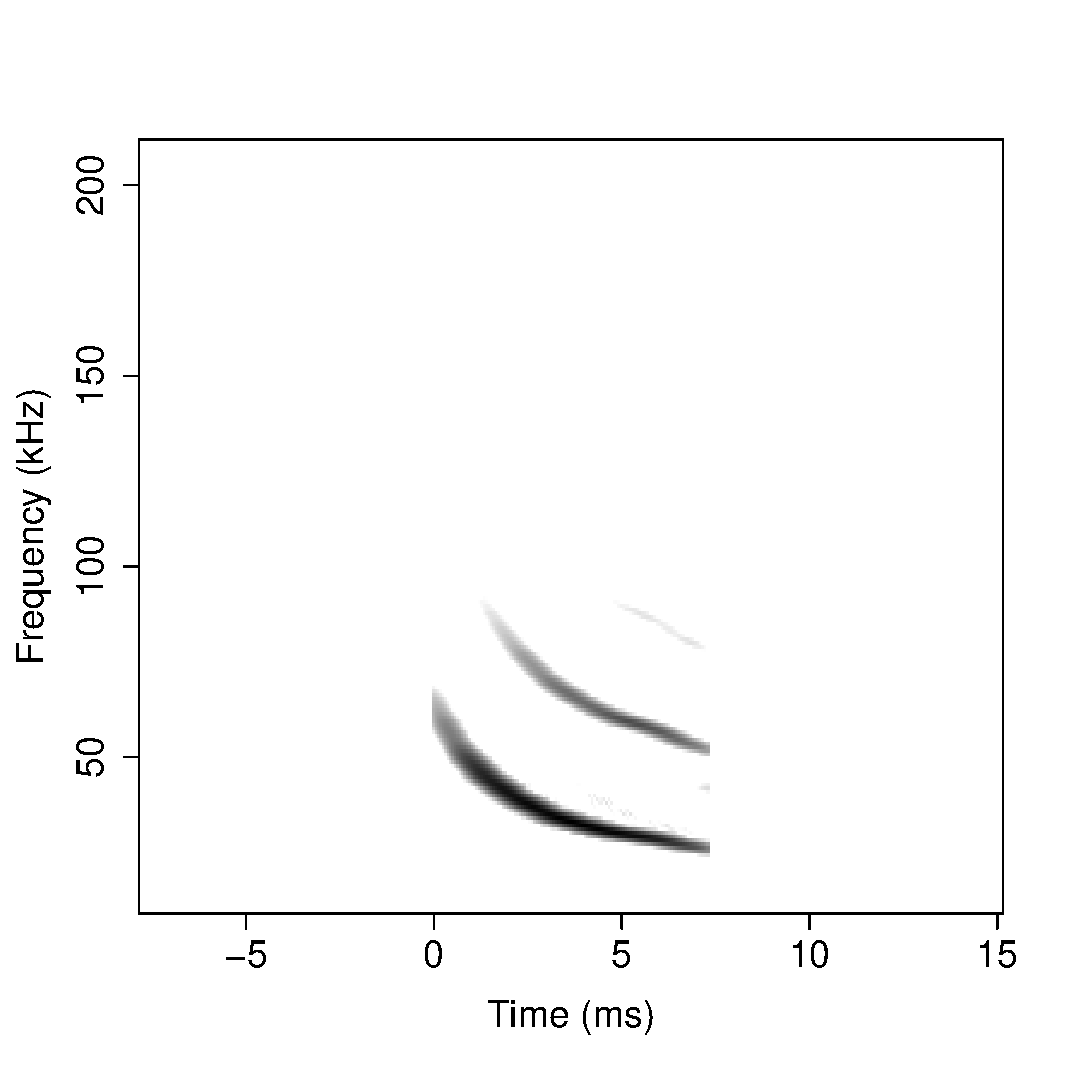
\includegraphics[width=1.5in]{../Figures/anpaSpectrogram.eps}\label{fig::anpa}}
		\hspace*{4pt}
		\subfigure[Narrowband, multiharmonic - \textit{Balantiopteryx plicata
		}]
		{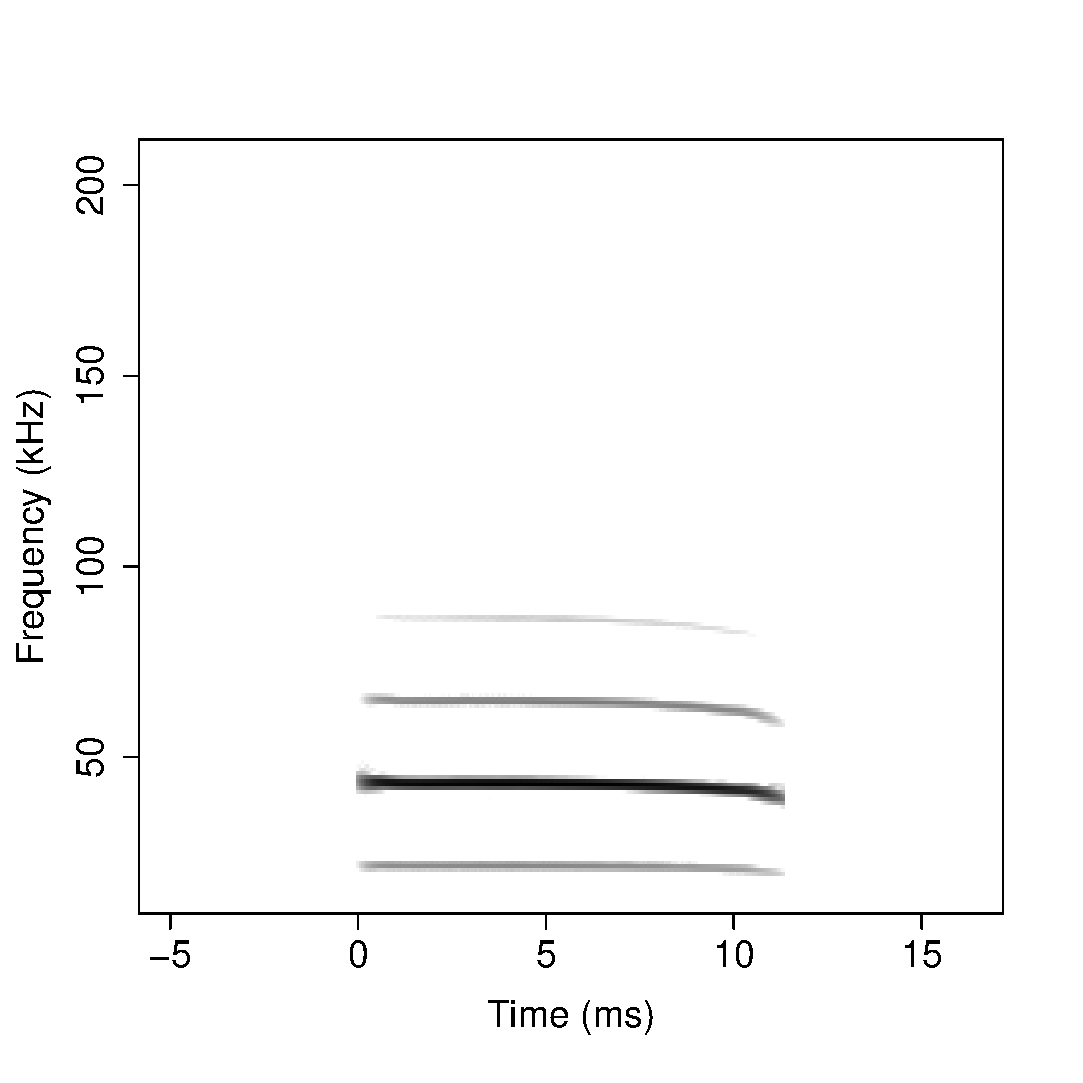
\includegraphics[width=1.5in]{../Figures/baplSpectrogram.eps}\label{fig::bapl}}
	}
	\centerline{
		\subfigure[Broadband sweep, single harmonic - \textit{Myotis yumanensis}]
		{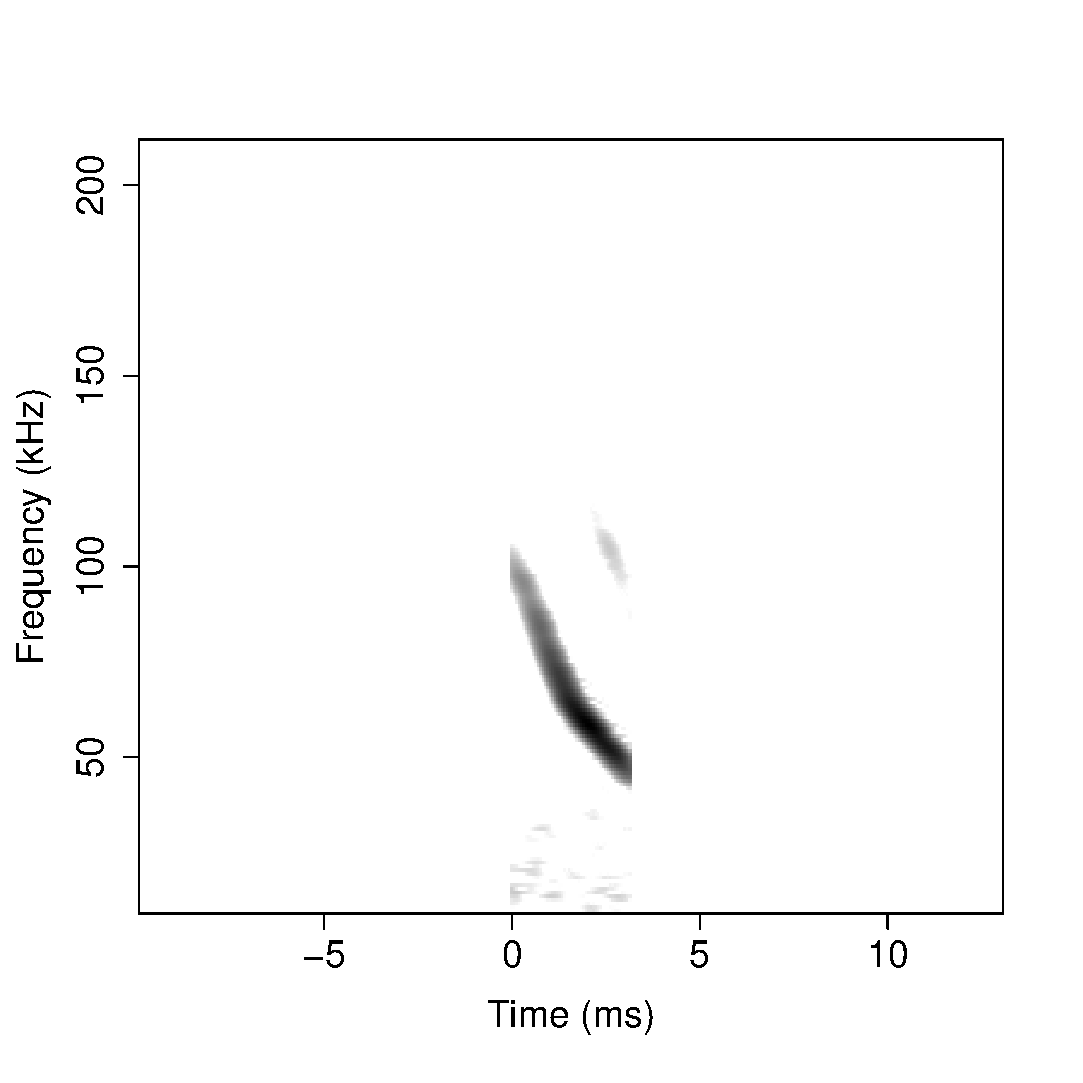
\includegraphics[width=1.5in]{../Figures/myyuSpectrogram.eps}\label{fig::myyu}}
		\hspace*{4pt}
		\subfigure[Constant frequency with broadband sweep - \textit{Pteronotus parnellii}]
		{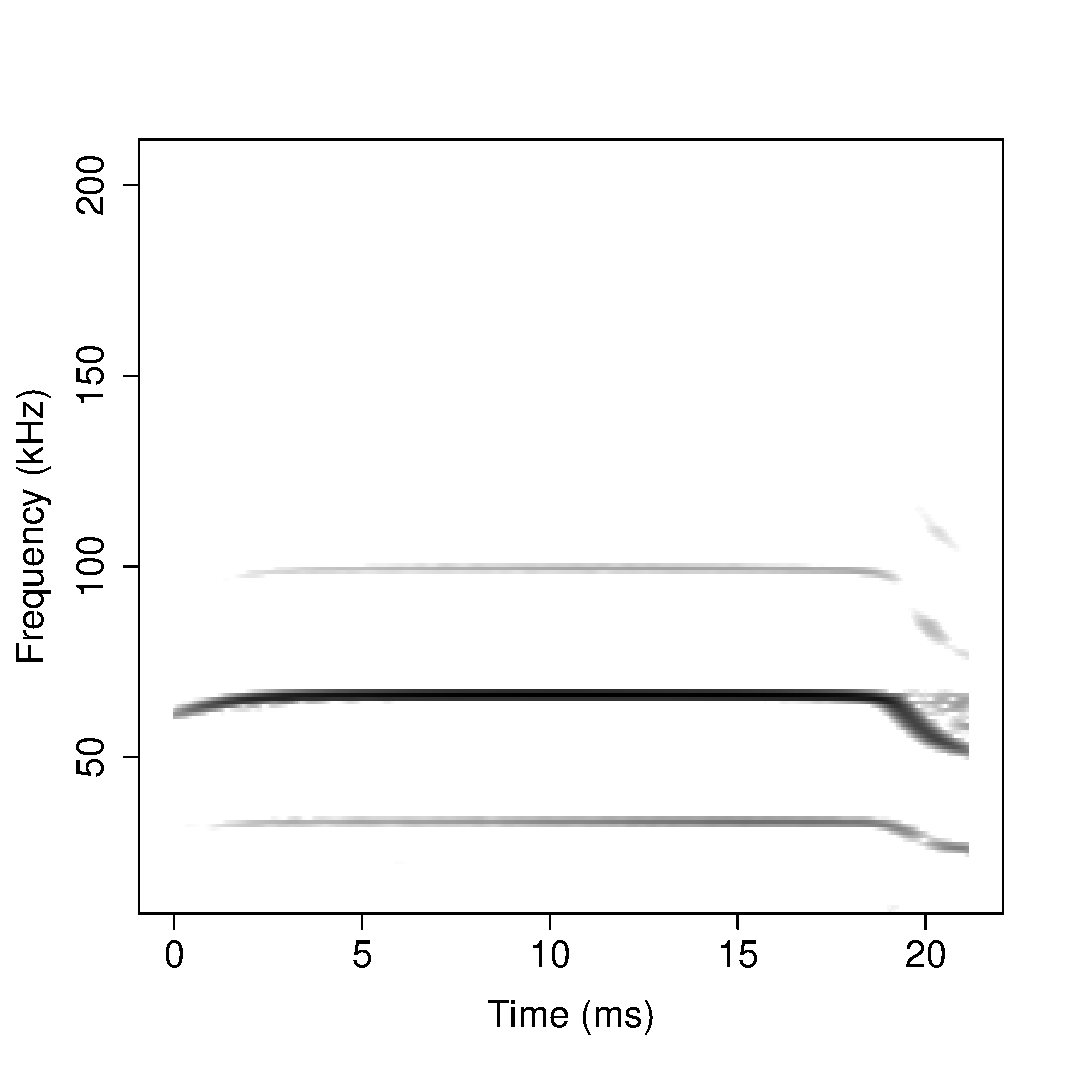
\includegraphics[width=1.5in]{../Figures/ptpaSpectrogram.eps}\label{fig::ptpa}}
	}
	\caption{Representative call spectrograms for some bat species, demonstrating echolocation call structures.}\label{fig::spectrogram}
\end{figure}
 
\subsection{Literature review}

Echolocation, or biosonar, is a process whereby sound is produced and the echoes that return from objects are used to perceive the environment.\cite{jones2005echolocation} Animals that use echolocation include bats, toothed whales, some birds, and some shrews and rats.\cite{jones2005echolocation} Bat echolocation calls, ranging from 9 to 212 kHz, differ from those of other echolocators in that they are often laryngeal, complex, and of a relatively long duration.\cite{thomas2004echolocation} The evolutionary dynamics that resulted in bats being nocturnal, flying echolocators have resulted in a wide variety of call structures across species.\cite{jones2006evolution} Echolocation in bats demonstrates convergent evolution, and bat species have been arranged in `guilds' based on habitat and foraging strategy, with similar call structures observed within a `guild'. \cite{aldridge1987morphology} \cite{neuweiler1990auditory} \cite{schnitzler2001echolocation} However, it has been acknowledged that ``echolocation signals reflect a phylogenetically determined basic call structure shaped by specific ecological conditions.''\cite{schnitzler2004evolution} Ancestral Reconstruction is a key aspect of understanding the variation is call structure that is due to phylogenetic relationships between species. 

Ancestral Reconstruction involves the extrapolation back in time from measured characteristics of current populations to the ancestral state, the estimate of the same characteristic in common ancestors.\cite{joy2016ancestral} Effective ancestral reconstruction relies on an accurate model for evolution, that is, both the dynamic evolutionary process and the phylogenetic relationships between species. \cite{joy2016ancestral} There have been maximum parsimony\cite{fitch1971toward}, maximum likelihood\cite{pupko2000fast}, and Bayesian\cite{pagel2004bayesian} approaches taken to ancestral reconstruction.

Other studies have considered bat echolocation calls for ancestral reconstruction. \cite{fenton1995signal} \cite{collen2012evolution}. Fenton\cite{fenton1995signal} hypothesised that early bats used short, broadband clicks for echolocation based on the observation that this is the method of echolocating employed by all animals except bats. Collen\cite{collen2012evolution} proposed instead that early bats used short, multi-harmonic, narrowband laryngeal calls for echolocation, based on a comparative analysis of echolocation call parameters. An approach to the reconstruction of early bat echolocation calls which is not so selective in the information it employs may shed further light on this topic. Gaussian Process Regression on Phylogenies for function valued traits provide a promising path to explore.\cite{jones2013evolutionary} Jones \& Moriarty proposed an extension to Gaussian Process Regression\cite{rasmussen2006gaussian} which allowed the generalisation of Ornstein-Uhlenbeck\cite{uhlenbeck1930theory} models of continuous-time character evolution for traits considered as functional data objects,\cite{ramsay2006functional} through a phylogeny. This study represents an effort to apply these methods to the ancestral reconstruction of bat echolocation calls.

\subsection{The evolution of function valued traits}

Bat echolocation calls can be described as 'function valued' traits.\cite{meyer2005up} In this context, 'function valued' refers to traits measured along a continuous scale, which can then be represented by a continuous mathematical function. Data of this nature can be viewed as functional data objects.\cite{ramsay2006functional} The Functional Phylogenies Group\cite{group2012phylogenetic} argue the case for performing evolutionary inference, including ancestral reconstruction, on function valued traits, with a particular focus on the evolution of linguistic speech sounds. They propose performing inference on a functional representation of the speech sound itself, by extending Gaussian Process Regression\cite{rasmussen2006gaussian} to take advantage of the tree structure of phylogenetic relationships.\cite{jones2013evolutionary}. 

Phylogenetic Gaussian Process Regression (PGPR), as developed by Jones \& Moriarty,\cite{jones2013evolutionary} extends Ornstein-Uhlenbeck\cite{uhlenbeck1930theory} models for continuous-time character evolution to function valued traits. In comparative studies of genetic data the O-U model is used to describe stabilising selection with random genetic drift, the notion that traits have some optimal value, around which they vary.\cite{hansen1997stabilizing} The PGPR is based on a kernel with 3 hyperparameters. Phylogenetic noise and length scale hyperparameters govern the correlation between nodes on a tree due to the phylogeny, while non-phylogenetic noise accounts for other sources of variation. Estimating these hyperparameters allows posterior distributions for traits at internal nodes to be constructed. In this way estimates for the ancestral state can be made. This model does not require that variance of the trait is homogenous across the whole function space. By defining a set of deterministic basis functions, combinations of which can be used to describe the observed trait functions, the variance of traits can be modelled to vary over the function space. An implementation of this method on simulated data is given by Hajipantelis.\cite{hadjipantelis2013function} 

\subsection{Paper Description}

In a similar manner to the representation of speech sounds as spectrograms,\cite{pigoli2015analysis} bat echolocation calls will be represented by their Energy Spectral Density\cite{antoniou2006digital} (ESD). The ESD, the energy of a signal as a function of a frequency, provides a straightforward characterisation from which a PGPR can be implemented. 

Using a synthetic dataset based on the bat phylogeny the conditions for an effective implementation of PGPR will be demonstrated. 

PGPR will then be implemented for the set of bat calls and posterior distributions of ESD estimated.

Spectral representations of the calls will be described, the implementation of PGPR. Independent Component Analysis. Simulations study to demonstrate the PGPR can work for this dataset. Application to Bats.

\section{Methods}

\subsection{Data Description}

The post processed echolocation call data accompanying Stathopoulos et al. \cite{stathopoulos2017bat} was used in this analysis. Echolocation calls were recorded across north and central Mexico with a Pettersson 1000x bat detector (Pettersson Elektronik AB, Uppsala, Sweden). Live trapped bats were measured and identified to species level using field keys.\cite{ceballos2005mamiferos} \cite{medellin2sanchez} Bats were recorded either while released from the hand or while tied to a zip line. The bat detector was set to record calls manually in real time, full spectrum at 500 kHz. 
In total the dataset consists of 22 species in five families, 449 individual bats and 1816 individual echolocation call recordings.

\begin{table}[ht]
	\tbl{Echolocation Call Dataset Statistics}
	{\begin{tabular}{@{}lccc@{}} \toprule
			Species & Key & Individuals & Calls \\ \colrule
			Family: Emballonuridae &&& \\
			1 \textit{Balantiopteryx plicata} & Bapl & 16 & 100 \\
			\\
			Family: Molossidae &&& \\
			2 \textit{Nyctinomops femorosaccus} & Nyfe & 16 & 100 \\
			3 \textit{Tadarida brasiliensis} & Tabr & 49 & 100  \\
			\\
			Family: Vespertilionidae &&& \\
			4 \textit{Antrozous pallidus} & Anpa & 58 & 100 \\
			5 \textit{Eptesicus fuscus} & Epfu & 74 & 100 \\
			6 \textit{Idionycteris phyllotis} & Idph & 6 & 100 \\
			7 \textit{Lasiurus blossevillii} & Labl & 10 & 90 \\
			8 \textit{Lasiurus cinereus} & Laci & 5 & 42 \\
			9 \textit{Lasiurus xanthinus} & Laxa & 8 & 100 \\
			10 \textit{Myotis volans} & Myvo & 8 & 100 \\
			11 \textit{Myotis yumanensis} & Myyu & 5 & 89 \\
			12 \textit{Pipistrellus hesperus} & Pihe & 85 & 100 \\
			\\
			Family: Mormoopidae &&& \\
			13 \textit{Mormoops megalophylla} & Mome & 10 & 100 \\
			14 \textit{Pteronotus davyi} & Ptda & 8 & 100 \\
			15 \textit{Pteronotus parnellii} & Ptpa & 23 & 100 \\
			16 \textit{Pteronotus personatus} & Ptpe & 7 & 51 \\
			\\
			Family:Phyllostomidae &&& \\
			17 \textit{Artibeus jamaicensis} & Arja & 11 & 82 \\
			18 \textit{Desmodus rotundus} & Dero & 6 & 38 \\
			19 \textit{Leptonycteris yerbabuenae} & Leye & 26 & 100 \\
			20 \textit{Macrotus californicus} & Maca & 6 & 53 \\
			21 \textit{Sturnira ludovici} & Stlu & 8 & 51 \\
			22 \textit{Sturnira lilium} & Stli & 4 & 20 \\
			\botrule
		\end{tabular}
	}
	\label{tab::dataset}
\end{table}

Phylogenetic relationships between species are described and dated according to the Bat super-tree produced by Collen.\cite{collen2012evolution} 

\begin{figure}
	\centering	q
	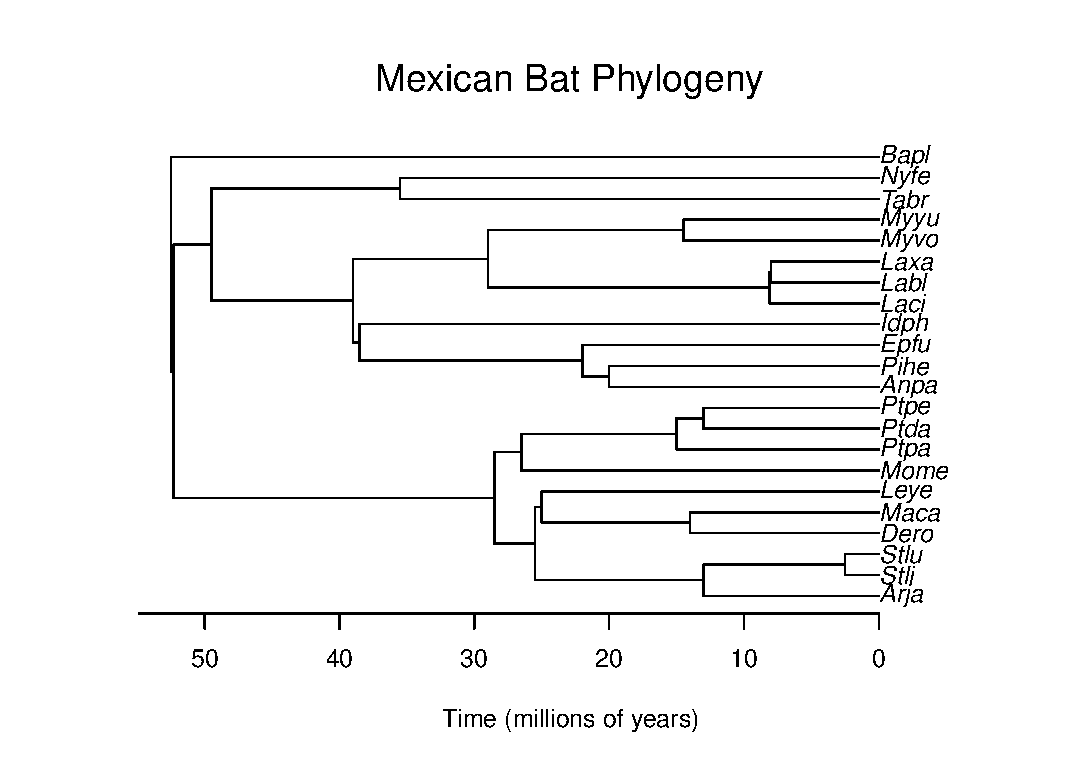
\includegraphics[width= 0.9\textwidth]{../Figures/Phylogeny.eps}
\end{figure}

\subsection{From Echolocation Call recordings to Spectral Curves}

Echolocation calls can be considered to be continuous, non-periodic, pulse signals which are a function of time \(x(t)\).

The Fourier Transform of a signal is an expression of the signal in the frequency domain, that is, as a function of frequency. It is given by 

\[
X(f) = \int_{-\infty}^{\infty} x(t) e^{-2\pi ft} dt.
\]

The energy of the signal is given by 

\[E = \int_{-\infty}^{\infty} |x(t)|^2 dt = \int_{-\infty}^{\infty} |X(f)|^2 df,\]

by Parseval's Theorem.

The ESD is then \(|X(f)|^2\). This is a representation of a sound and so it is appropriate to scale this to a decibel scale. Not also that \(|X(f)|^2\) is a periodic function and symmetric around 0. Given that bat echolocation calls range from \(9 - 212\)kHz we are interested in \(S(f) = log_{10} |X(f)|^2, f \in [9, 212] \). This can then be treated as a functional data object.

By treating \(S(f)\) as a functional data object it is treated as a set of noisy realisations taken of a smooth underlying curve. Estimating this underlying curve is performed by smoothing. Another aspect of functional data analysis is registration, in this case it would consist of separating out phase and amplitude variation. As the energy at specific frequencies is of interest here, registration along the frequency axis is not appropriate. However the level of the amplitude depends on factors such as the distance of the bat from the microphone while being recorded. This variation is not interesting. Thus registration on the amplitude axis is appropriate. thus all curves are registered such that the amplitude lies on the interval \([0,1]\). 

Once smoothed and registered the curves are sampled from at every kHz. These Spectral curves are the functions to be analysed in the comparative analysis.

\subsection{Phylogenetic Gaussian Process Regression for spatially inhomogenous data}

Some stuff about Gaussian Process Regression

Extension of Gaussian Processes to Phylogenetic Data

Extension to spatially inhomogenous data.

The theoretical results presented by Jones \& Moriarty\cite{jones2013evolutionary} rely on two assumptions about the data

\subsection{Component Analysis}

PCA and ICA execution. Tuning of components.

\subsection{Phylogenetic Gaussian Processes}

Gaussian Processes, Matern / OU kernel, interpretation of parameters

proceedings 

\section{Results}

\subsection{Simulation Study}

given hypers, what happens along the given tree

\subsection{Mexican Bat Echolocation call Dataset}

What happens when the method is applied to the Mexican bat calls?

\section{Discussion}

\subsection{What do we learn from this?}

Phylogenetic / Non-phylogenetic Signal. Not just noise. Although speculative and probably limited going back to root may be useful for more recent ancestors.

\subsection{Future Work in this Area}

Implement for Spectrograms, produce some recordings.


\bibliographystyle{ws-rv-van}
\bibliography{../BatBiblio}

%\blankpage
%\printindex[aindx]                 % to print author index
%\printindex                         % to print subject index

\end{document} 